Um ein besseres Verständnis zu ermöglichen, wird zunächst auf die generelle Funktionsweise von Maven näher eingegangen. 
\dwi{ich sags nur ungern, aber das hier ist wieder ein ausflug bei dem du in der arbeit mitteilst was du über maven gelernt hast, ohne das es die kernaussagen deiner 
arbeit notwendig machen würden. ich empfehle einen durchgang mit rotstift.}

\subsubsection{Workflow Maven}
Maven verfolgt die Philosopie \textit{Konvention über Konfiguration}. 

In diesem Rahmen sind Strukuren oder Abläufe, die zur Kompilierung, Testen, Paketierung und Veröffentlichung von Projekten benötigt werden, bereits vorgegeben und müssen nicht mehr definiert werden, wodurch sich die Entwicklung auf den Inhalt des Projektes einschränkt. \cite[S. 27]{spiller_maven_2011}

Softwareentwickler werden unterstützt, indem Maven die Ordnerstruktur und Organisation eines Projektes standardisiert und Empfehlungen abgibt, wo sich verschiedene Teile des Codes wie der Quellcode oder Konfigurationsdateien abgelegt werden sollten. \cite[S. 2]{varanasi_introducing_2019}  

Ferner bietet Maven die Möglichkeit Projektabhängigkeiten, Projektumgebungen und Projektbeziehungen in einer seperaten, externen pom.xml-Datei zu deklarieren. \cite[S. 3]{varanasi_introducing_2019} 

Dies erleichtert insbesondere die Verwaltung von Projektabhängigkeiten, da Bibliotheken einfach ausgetauscht werden können und die entsprechenden Abhängigkeiten sowie die transitiven Abhängigkeiten aufgelöst und entfernt werden.

Aufgrund der vielen automatisierten und standardisierten Schritte insbesondere im Bereich des Build-Managements, wird die Navigation übersichtlich und das Verständnis erheblich erleichtert. 

\begin{figure}[h]
    \centering
    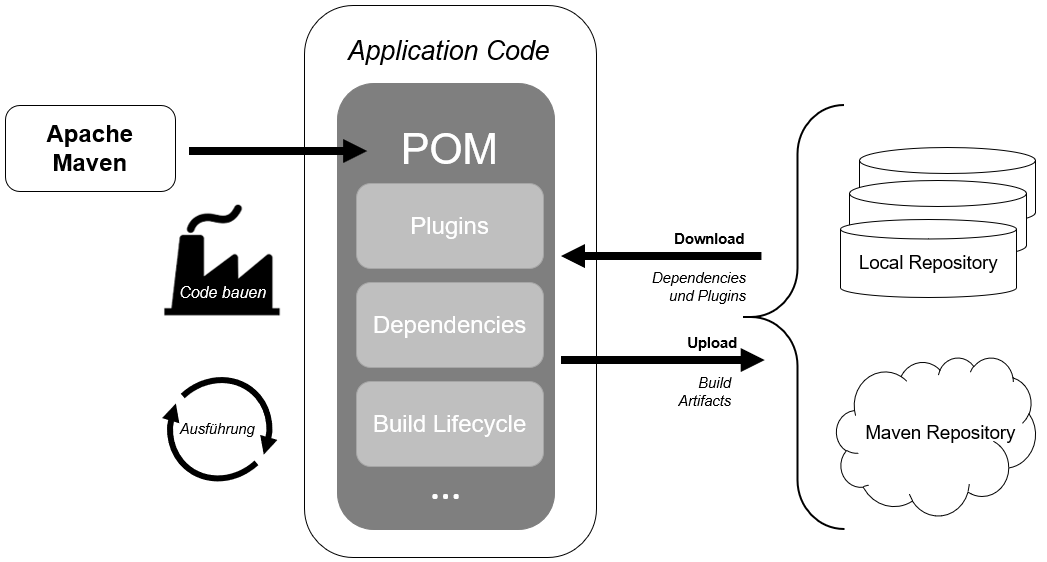
\includegraphics[scale=0.6]{Bilder/Workflow_Maven.png}
    \caption{Funktionsweise von Maven, angelehnt an \cite{guntur_understanding_2020}}
\end{figure}

\paragraph{POM}
Die Funktionsweise von Maven als auch die Verwaltung des Projektes baut grundsätzlich auf dem 'Project Object Model' (kurz: POM) auf und bildet daher den Kern eines jeden Maven-Projektes ab.

Die POM wird innerhalb der Datei pom.xml gespeichert, die wiederrum im Projektverzeichnis liegt.

Die POM beinhaltet alle notwendigen Projektinformationen, vorhandenen Abhängigkeiten, dem Quelldateiverzeichnis Konfigurationen und Plugininformationen, die während des Build-Prozesses verwendet werden sollen.\cite{the_apache_software_foundation_maven_2002}

Die POM muss drei wesentliche Tags enthalten \cite[S. 77 - 78]{spiller_maven_2011}: 

\begin{itemize}
    \item \textit{groupId}: Enthält eine eindeutige, identifizierbare Bezeichnung für ein Projekt
    \item \textit{artifactId}: Enthält eine eindeutige, identifizierbare Bezeichnung für ein Artefakt bzw. Projekt pro groupId
    \item \textit{version}: Enthält die aktuelle Version des Artefakts
\end{itemize}

Alle weiteren definierten Eigenschaften werden von der Super-POM vererbt, welches die Standardkonfigurationen, Plugins und Verzeichnisse enthält.

Entscheidend ist, dass Maven keine vollständigen Projekte, sondern eigenständige Projektteile, also Artefakte beschreibt, die einzeln ausgeliefert werden. \cite[S. 29]{spiller_maven_2011}

Demzufolge erzeugt jedes Maven-Projekt ein Artefakt, welches auf die Repositorys übertragen wird. 

\paragraph{Repository}

Ferner verwendet Maven das 'Local Repository' und das konfigurierte 'Maven Repository'.

Innerhalb des Local Repositorys werden alle Abhängigkeiten abgelegt, die für die Erstellung des Builds benötigt werden. 

Zunächst überprüft Maven bei der Zerlegung der Abhängigkeiten, ob sich die benötigten Dateien bereits innerhalb des Local Repositorys befinden. \cite[S. 45 - 47]{loukides_maven_2008} 

Ist dies der Fall, wird die Datei, ohne die Erstellung einer Kopie im lokalen Verzeichnis, innerhalb des Local Repositorys verwendet.

Kann keine Zerlegung der Abhängigkeiten lokal erfolgen, versucht Maven diese mittels dem Maven Repository über das Internet auf das Local Repository herunterzuladen und zu kopieren, damit diese aussschließlich lokal verwendet werden. \cite[S. 115]{spiller_maven_2011}   

Sollten neue Abhängigkeiten oder neue Versionen der vorhandenen Abhängigkeiten hinzugefügt werden, wird das Repository anhand dessen aktualisiert oder die betreffenden Abhängigkeiten kopiert. 

Die Abhängigkeiten, also die genutzten Bibliotheken werden in der pom.xml definiert. 

\paragraph{Build-Lifecycle}

Prinzipiell sind Lifecycles abstrahierte Arbeitsschritte innerhalb festen Phasen, die in einer bestimmten Reihenfolge durchlaufen und für den Build-Prozess essentiell sind. \cite[S. 57]{varanasi_introducing_2019}  

Durch das standardisierte Vorgehen, lässt sich das Ararbeiten der Aufgaben verallgemeinern und vereinheitlichen, was für den Entwickler unterstützend ist.

Maven definiert dabei drei Lifecycles\cite[S. 72 - 76]{spiller_maven_2011}: 

\begin{itemize}
    \item \textit{clean}\\
    Mittels dieses Lifecycles wird alles gelöscht, was keine Notwendigkeit mehr hat, so wie beispielsweise die vom vorherigen Build erstellten Dateien. 

    \item \textit{site}\\
    Innerhalb dieses Lifecycles umfasst alle Phasen, die zum Erzeugen einer Projektdokumentation benötigt werden.
    
    \item \textit{build/default}\\
    Dieser Lifecycle stellt den standardisierten Ablauf aller Phasen dar, die nach dem Aufruf von Maven zum Übersetzen und Erzeugen einer Anwendung abgearbeitet werden. 
    
    Dieser enthält acht wesentliche Phasen, die nach einer unveränderbaren Reihenfolge abgearbeitet werden: validate, compile, test, package, integration-test, verify, install und deploy.  

\end{itemize}

Folglich muss bei einem Aufruf einer bestimmten Phase, die vorangegangen Phasen ebenfalls abgearbeitet werden. 

Neben den Phasen sind auch die zugrundeliegenden Plugins innerhalb jedes Lifecycles verbunden, die sich wiederrum durch das Ausführen von Plugin-Goals in den einzelnen Phasen modefizieren lassen. \cite[S. 71]{spiller_maven_2011}

\begin{figure}[h]
    \centering
    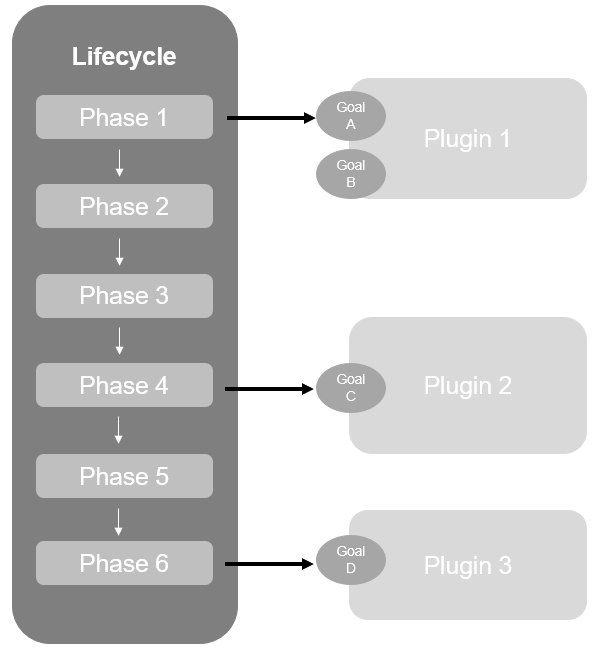
\includegraphics[scale=0.5]{Bilder/lifecycle_maven.png}
    \caption{Zusammenspiel Plugin-Goals und Lifecycle, \cite[S. 59]{varanasi_introducing_2019}}
\end{figure}

Sobald Maven die einzelnen Phasen eines Lifecycles durchläuft, werden die Ziele ausgeführt, die mit jeder einzelnen Phase verbunden sind. \cite[S. 39]{loukides_maven_2008} 

Infolgedessen werden bestimmte Funktionalität eines Plugins durch das entsprechende Goal bestimmt. 

Während das POM alle notwendigen Informationen über ein Projekt enthält, die während des Build-Prozesses verwendet werden sollen, also das "Wer", "Was" und "Wo", stellt der Lifecycle das "Wann" und "Wie" dar. \cite{the_apache_software_foundation_maven_2002}

\paragraph{Plugins in Maven}

Wie bereits beschrieben, ist Maven ein Framework zum Ausführen von Plugins, indem benötigte Funktionen als Plugins anhand des Goals in den Softwareentwicklungsprozess ausgeführt werden.

In diesem Rahmen wird das Konzepts \textit{Seperation of Concerns} verfolgt. 

Aufgrund der hohen Anzahl der Varianten derselben Funktionalitäten wie beispielsweise das Kompilieren oder das Testen, muss stets ein Goal innerhalb eines Plugins angegeben werden, wodurch ein Maven-Plugin für genau eine Aufgabe zuständig ist. 

Infolgedessen kann jede Funktionalität durch ein Plugin ersetzt werden, wodurch Plugins eine zentrale Rolle innerhalb des Softwareentwicklungsprozesses zufällt. 

Wird das Plugin regelmäßig verwendet, wird dieses innerhalb der POM deklariert, ansonsten reicht ein Aufruf über die Kommandozeile.  

Durch die Koordinaten groupId, artifactId und version können die Artefakte identifiziert werden, wobei die Verwaltung der Abhängigkeiten ebenfalls im Repository erfolgt. 

Mittels der Auslagerung unterschiedlicher Aufgaben, ist sowohl der Einsatz als auch die Wartung einfacher wie bei großen Abhängigkeiten, da die Aktualisierung durch Maven durchgeführt werden.  

\subsubsection{Entwurf des PoC basierend auf dem Ayoy - Maven Licence Vertify Plugin}

Kernelement des Ayoy-Plugins ist die Prüfung und der darauf aufbauende Vergleich von Lizenzmodellen und deren Abhängigkeiten innerhalb eines Projektes.

\begin{figure}[h]
    \centering
    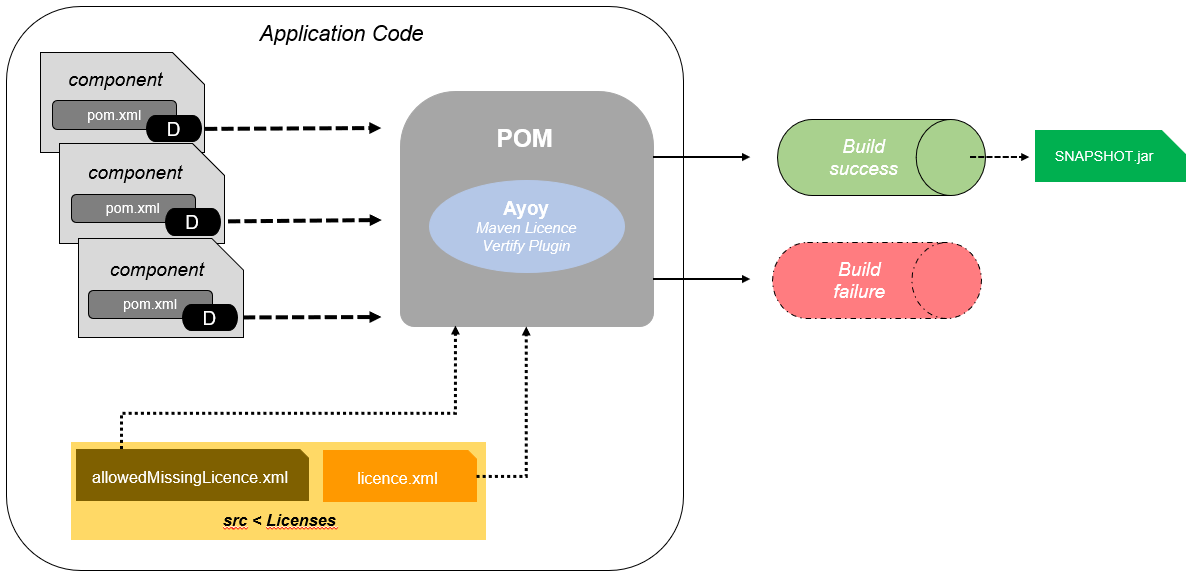
\includegraphics[scale=0.4]{Bilder/Ayoy-Plugin.png}
    \caption{Funktionsweise des Ayoy-Plugin}
\end{figure}
\dwi{alert! JEDE grafik, die du in den text einbaust und NICHT explizit im text referenzierst (wie das geht hab ich dir schonmal gezeigt) werde ich als überflüssig betrachten und nicht anschauen. falls du das nicht mehr weißt, andreas hessenthaler kann dir das auch schnell nochmal zeigen.}

Alle Komponeten des ausführbaren Programms beinhalten zunächst jeweils eine pom.xml-Datei und die darin enthaltenen Bibliotheken als zu prüfende Abhängigkeiten. 

Eine pom.xml enthält neben der groupId, artifactId und version zur Identifikation, die Lizenz des Projektes, verschiedene Abhängigkeiten und die entsprechenden Plugins, die zur Ausführung benötigt werden.  

Die für den Vergleich essentielle licence.xml und befindet sich src-Verzeichnis.  
\dwi{welches src-verzeichnis? vom program? muss ich in dieser lösung in JEDEM programm eine solche datei hinterlegen? das solltest du hier sehr genau beschreiben.}

Die darin enthaltenen Lizenzmodelle werden jeweils mit Namen und der dazu gehörigen URL versehen. 

Die Angabe der URL muss zwingend eingehalten werden, da der Vergleich auf diesem Wert basiert, während der Name aussschließlich für die Ausgabe verwendet wird.
\dwi{was passiert, wenn eine license.xml die URL nicht enthält?}

Die licence-Datei wird als ein xml-Format gespeichert und enthält alle erlaubten ('valid') und nicht genehmigten ('forbidden') Lizenzmodelle. 

\begin{figure}[h]
    \centering
    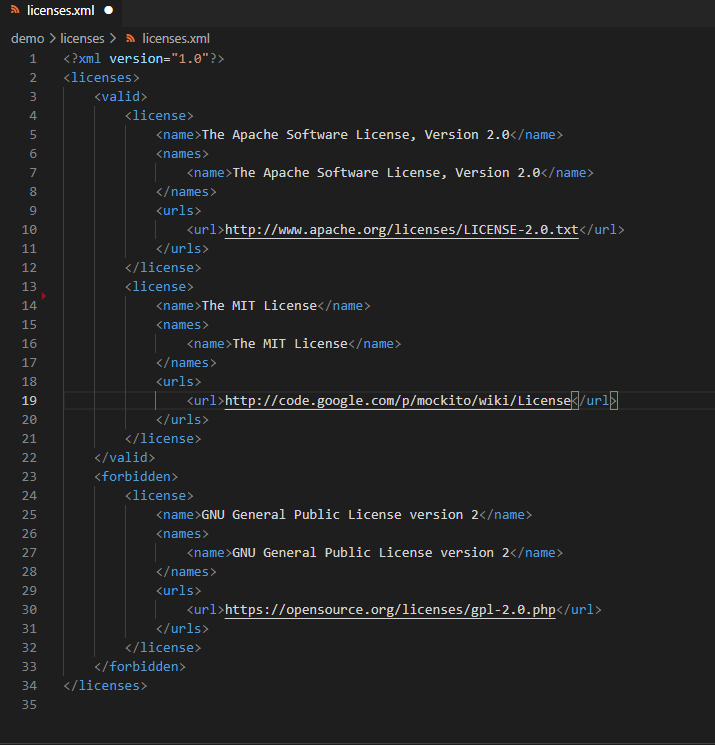
\includegraphics[scale=0.45]{Bilder/licencesxml.png}
    \caption{Genehmigte und nicht genehmigte Lizenzmodelle innerhalb der licence.xml}
\end{figure}

Nachdem der Build-Prozess angestoßen wird, vergleicht das Plugin alle Lizenzen der unterschiedlichen pom.xml-Dateien und deren Abhängigkeiten des aktuellen Projekts mit der entsprechenden licence.xml. 

Wenn die Anforderungen erfüllt sind, wird der Build-Prozess erfolgreich ausgeführt, ansonsten wird dieser abgebrochen. 

Ferner kann der Build-Prozess unterschiedlich gestartet werden. 

Sollte das Plugin, gemäß der Anforderungsdefinition, automatisiert und daher regelmäßig durchgeführt werden, muss der entsprechende Aufruf innerhalb der pom.xml eingebettet werden. 

\begin{figure}[h]
    \centering
    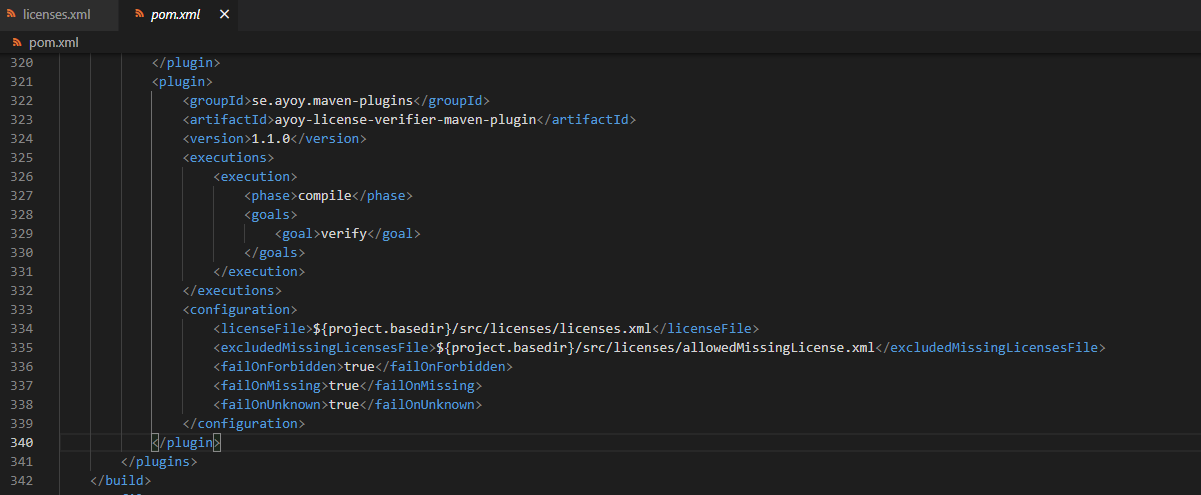
\includegraphics[scale=0.5]{Bilder/PluginConfigurationzumAufruf.png}
\end{figure}

Bei unregelmäßiger Verwendung kann der Aufruf über die Kommandozeile mittels folgenden Befehl eingegeben werden:  

\begin{figure}[h]
    \centering
    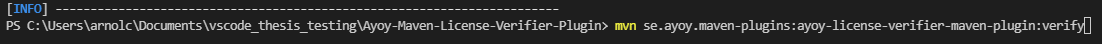
\includegraphics[scale=0.5]{Bilder/mvn-Aufruf.png}
\end{figure}

Der Aufruf spiegelt den Pfad des Goals des Plugins innerhalb des Repositorys dar: 

\begin{itemize}
    \item \textbf{mvn}: Syntax zum Ausführen des Maven-Befehls
    \item \textbf{se.ayoy.maven-plugins}: Aufruf der Bibliothek innerhalb des Repositorys
    \item \textbf{ayoy-license-verifier-maven-plugin}: Aufruf des Plugins auf dem Repositorys
    \item \textbf{verify}: Goal des Plugins
\end{itemize}

Die Prüfung der Abhängigkeiten ist neben der Prüfung der direkten Lizenzen von Komponenten essentiell, da Bibliotheken ebenfalls Lizenzmodelle besitzen, die ein starkes Copyleft aufweisen können und aufgrund dessen von dem Plugin erkannt werden müssen. 

Auch können Abhängigkeiten eingebunden werden, die weitere Abhängigkeiten aufweisen und diese widerrum ein risikoreiches Copyleft aufweisen. 
\dwi{die fähigkeit, transitive abhängigkeiten zu prüfen sollte eine funktionale anforderung sein, oder? :-)}

Ferner besteht die Möglichkeit, dass sich die Lizenzen der Abhängigkeiten aufgrund einer Versionsänderung auf ein Lizenmodel mit beschränkter oder starker Copyleft umgestellen.  

Sowohl Versionumstellungen \dwi{Versionsumstellungen} als auch transitive Abhängigkeiten sind oftmals für den Entwickler nicht sofort erkennbar und bieten ein hohes Potential 'gefährliche' Lizenzmodelle zu übersehen. 

Während diese Abhängigkeiten zwingend betrachtet werden müssen, sollten Abhängigkeiten die aussschließlich zum Testen verwendet werden, sowie bereits in Szenario eins beschrieben, nicht innerhalb des Plugins einbezogen werden. 

Da diese Abhängigkeiten aussschließlich für Testzwecke verwendet und folglich nicht ausgeliefert werden, ist eine Beachtung der Lizenzmodelle nicht zwingend notwendig. 

\begin{figure}[h]
    \centering
    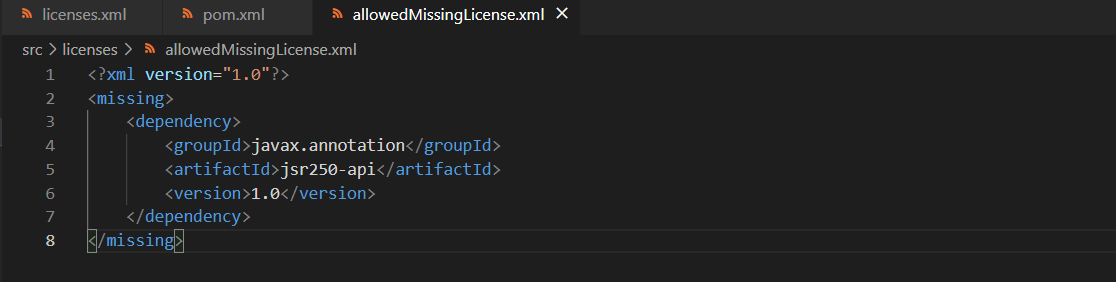
\includegraphics[scale=0.5]{Bilder/allowedmiisingLicence.png}
\end{figure}

Zu diesem Zweck müssen die entsprechenden Lizenzen zunächst innerhalb der allowedMissingLicence.xml eingebettet werden.
\dwi{ich bin mir unsicher, ob dies (=testen) der originalzweck dieser XML datei ist. das legst du dem leser mit der vorigen argumentation aber nahe. hier vielleicht nachschärfen.}

Die Lizenzmodelle der darin eingegebenen Abhängigkeiten werden vom Plugin ignoriert, ohne das Build-Prozess fehlschlägt, falls eine risikoreiche Lizenzen gefunden wird. 

Als Ergebnis des Build-Prozesses wird die SNAPSHOT.jar als eine ausführbare Datei erstellt. 
















